\documentclass{standalone}

\usepackage[english]{babel}
\usepackage[utf8]{inputenc}
\usepackage[T1]{fontenc}

\usepackage{amsmath, amssymb}

\usepackage{tikz}

\begin{document}

    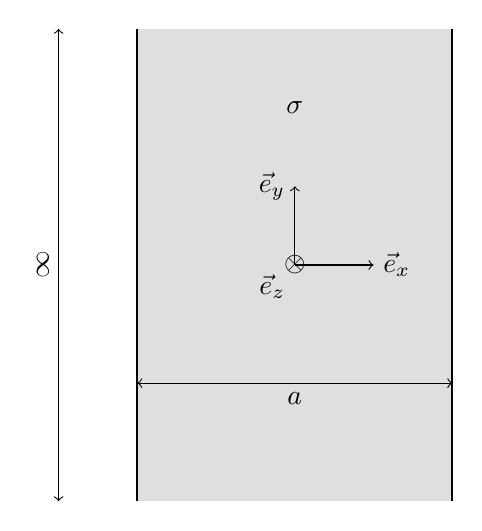
\begin{tikzpicture}
        \pgfmathsetmacro{\sizeX}{4}
        \pgfmathsetmacro{\sizeY}{6}

        \fill[color=gray!25!white] (-\sizeX/2, -\sizeY/2) rectangle
            (\sizeX/2, \sizeY/2);

        \draw[->] (0, 0) -- (1, 0) node[right] {$\vec{e}_x$};
        \draw[->] (0, 0) -- (0, 1) node[left] {$\vec{e}_y$};
        \draw (0, 0) node {$\otimes$} node[below left] {$\vec{e}_z$};

        \draw[-, thick] (-\sizeX/2, -\sizeY/2) -- ++(0, \sizeY);
        \draw[-, thick] (\sizeX/2, -\sizeY/2) -- ++(0, \sizeY);

        \draw[<->] (-\sizeX/2, -1.5) -- node[below] {$a$} ++(\sizeX, 0);
        \draw[<->] (-\sizeX/2 - 1, -\sizeY/2) --node[above, sloped] {$\infty$}
            ++(0, \sizeY);

        \draw (0, 2) node {$\sigma$};

    \end{tikzpicture}

\end{document}
